\documentclass[a4paper]{article}

\usepackage{inputenc}
\usepackage[british,UKenglish]{babel}
\usepackage{amsmath}
%\usepackage{titlesec}
\usepackage{color}
\usepackage{graphicx}
\usepackage{fancyref}
\usepackage{hyperref}
\usepackage{float}
\usepackage{scrextend}
\usepackage{setspace}
\usepackage{xargs}
\usepackage{multicol}
\usepackage{nameref}

\usepackage{sectsty}
\usepackage{multicol}
\usepackage{multirow}
\usepackage[procnames]{listings}
\usepackage{appendix}

\newcommand\tab[1][1cm]{\hspace*{#1}}
\hypersetup{colorlinks=true, linkcolor=black}
\interfootnotelinepenalty=10000

\newcommand{\cleancode}[1]{\begin{addmargin}[3em]{3em}\texttt{\textcolor{cleanOrange}{#1}}\end{addmargin}}
\newcommand{\cleanstyle}[1]{\text{\textcolor{cleanOrange}{\texttt{#1}}}}


\usepackage[colorinlistoftodos,prependcaption,textsize=footnotesize]{todonotes}
\newcommandx{\commred}[2][1=]{\textcolor{Red}
{\todo[linecolor=red,backgroundcolor=red!25,bordercolor=red,#1]{#2}}}
\newcommandx{\commblue}[2][1=]{\textcolor{Blue}
{\todo[linecolor=blue,backgroundcolor=blue!25,bordercolor=blue,#1]{#2}}}
\newcommandx{\commgreen}[2][1=]{\textcolor{OliveGreen}{\todo[linecolor=OliveGreen,backgroundcolor=OliveGreen!25,bordercolor=OliveGreen,#1]{#2}}}
\newcommandx{\commpurp}[2][1=]{\textcolor{Plum}{\todo[linecolor=Plum,backgroundcolor=Plum!25,bordercolor=Plum,#1]{#2}}}

\def\code#1{{\tt #1}}

\def\note#1{\noindent{\bf [Note: #1]}}

\makeatletter
%% The "\@seccntformat" command is an auxiliary command
%% (see pp. 26f. of 'The LaTeX Companion,' 2nd. ed.)
\def\@seccntformat#1{\@ifundefined{#1@cntformat}%
   {\csname the#1\endcsname\quad}  % default
   {\csname #1@cntformat\endcsname}% enable individual control
}
\let\oldappendix\appendix %% save current definition of \appendix
\renewcommand\appendix{%
    \oldappendix
    \newcommand{\section@cntformat}{\appendixname~\thesection\quad}
}
\makeatother


% "define" Scala
\usepackage[T1]{fontenc}  
\usepackage[scaled=0.82]{beramono}  
\usepackage{microtype} 

\sbox0{\small\ttfamily A}
\edef\mybasewidth{\the\wd0 }

\lstdefinelanguage{scala}{
  morekeywords={abstract,case,catch,class,def,%
    do,else,extends,false,final,finally,%
    for,if,implicit,import,match,mixin,%
    new,null,object,override,package,%
    private,protected,requires,return,sealed,%
    super,this,throw,trait,true,try,%
    type,val,var,while,with,yield},
  sensitive=true,
  morecomment=[l]{//},
  morecomment=[n]{/*}{*/},
  morestring=[b]",
  morestring=[b]',
  morestring=[b]"""
}

\usepackage{color}
\definecolor{dkgreen}{rgb}{0,0.6,0}
\definecolor{gray}{rgb}{0.5,0.5,0.5}
\definecolor{mauve}{rgb}{0.58,0,0.82}

% Default settings for code listings
\lstset{frame=tb,
  language=scala,
  aboveskip=3mm,
  belowskip=3mm,
  showstringspaces=false,
  columns=fixed, % basewidth=\mybasewidth,
  basicstyle={\small\ttfamily},
  numbers=none,
  numberstyle=\footnotesize\color{gray},
  % identifierstyle=\color{red},
  keywordstyle=\color{blue},
  commentstyle=\color{dkgreen},
  stringstyle=\color{mauve},
  frame=single,
  breaklines=true,
  breakatwhitespace=true,
  procnamekeys={def, val, var, class, trait, object, extends},
  procnamestyle=\ttfamily\color{red},
  tabsize=2
}

\lstnewenvironment{scala}[1][]
{\lstset{language=scala,#1}}
{}
\lstnewenvironment{cpp}[1][]
{\lstset{language=C++,#1}}
{}
\lstnewenvironment{bash}[1][]
{\lstset{language=bash,#1}}
{}
\lstnewenvironment{verilog}[1][]
{\lstset{language=verilog,#1}}
{}



%代码段设置
\lstset{numbers=left,
basicstyle=\tiny,
numberstyle=\tiny,
keywordstyle=\color{blue!70},
commentstyle=\color{red!50!green!50!blue!50},
frame=single, rulesepcolor=\color{red!20!green!20!blue!20},
escapeinside=``
}

\graphicspath{ {images/} }
\usepackage{ctex}
\usepackage{graphicx}
\usepackage{color,framed}%文本框
\usepackage{listings}
\usepackage{caption}
\usepackage{amssymb}
\usepackage{enumerate}
\usepackage{xcolor}
\usepackage{bm} 
\usepackage{lastpage}%获得总页数
\usepackage{fancyhdr}
\usepackage{tabularx}  
\usepackage{geometry}
\usepackage{minted}
\usepackage{graphics}
\usepackage{subfigure}
\usepackage{float}
\usepackage{pdfpages}
\usepackage{pgfplots}
\pgfplotsset{width=10cm,compat=1.9}
\usepackage{multirow}
\usepackage{footnote}
\usepackage{booktabs}

%-----------------------伪代码------------------
\usepackage{algorithm}  
\usepackage{algorithmicx}  
\usepackage{algpseudocode}  
\floatname{algorithm}{Algorithm}  
\renewcommand{\algorithmicrequire}{\textbf{Input:}}  
\renewcommand{\algorithmicensure}{\textbf{Output:}} 
\usepackage{lipsum}  
\makeatletter
\newenvironment{breakablealgorithm}
  {% \begin{breakablealgorithm}
  \begin{center}
     \refstepcounter{algorithm}% New algorithm
     \hrule height.8pt depth0pt \kern2pt% \@fs@pre for \@fs@ruled
     \renewcommand{\caption}[2][\relax]{% Make a new \caption
      {\raggedright\textbf{\ALG@name~\thealgorithm} ##2\par}%
      \ifx\relax##1\relax % #1 is \relax
         \addcontentsline{loa}{algorithm}{\protect\numberline{\thealgorithm}##2}%
      \else % #1 is not \relax
         \addcontentsline{loa}{algorithm}{\protect\numberline{\thealgorithm}##1}%
      \fi
      \kern2pt\hrule\kern2pt
     }
  }{% \end{breakablealgorithm}
     \kern2pt\hrule\relax% \@fs@post for \@fs@ruled
  \end{center}
  }
\makeatother
%------------------------代码-------------------
\usepackage{xcolor} 
\usepackage{listings} 
\lstset{ 
breaklines,%自动换行
basicstyle=\small,
escapeinside=``,
keywordstyle=\color{ blue!70} \bfseries,
commentstyle=\color{red!50!green!50!blue!50},% 
stringstyle=\ttfamily,% 
extendedchars=false,% 
linewidth=\textwidth,% 
numbers=left,% 
numberstyle=\tiny \color{blue!50},% 
frame=trbl% 
rulesepcolor= \color{ red!20!green!20!blue!20} 
}

%-------------------------页面边距--------------
\geometry{a4paper,left=2.3cm,right=2.3cm,top=2.7cm,bottom=2.7cm}
%-------------------------页眉页脚--------------
\usepackage{fancyhdr}
\pagestyle{fancy}
\lhead{\kaishu \leftmark}
% \chead{}
\rhead{\kaishu 数据库实验报告}%加粗\bfseries 
\lfoot{}
\cfoot{\thepage}
\rfoot{}
\renewcommand{\headrulewidth}{0.1pt}  
\renewcommand{\footrulewidth}{0pt}%去掉横线
\newcommand{\HRule}{\rule{\linewidth}{0.5mm}}%标题横线
\newcommand{\HRulegrossa}{\rule{\linewidth}{1.2mm}}
\setlength{\textfloatsep}{10mm}%设置图片的前后间距
%--------------------文档内容--------------------

\begin{document}
\renewcommand{\contentsname}{目\ 录}
\renewcommand{\appendixname}{附录}
\renewcommand{\appendixpagename}{附录}
\renewcommand{\refname}{参考文献} 
\renewcommand{\figurename}{图}
\renewcommand{\tablename}{表}
\renewcommand{\today}{\number\year 年 \number\month 月 \number\day 日}

%-------------------------封面----------------
\begin{titlepage}
    \begin{center}
    
\includegraphics[width=0.8\textwidth]{NKU.png}\\[1cm]
    \vspace{20mm}
		\textbf{\huge\textbf{\kaishu{计算机学院}}}\\[0.5cm]
		\textbf{\huge{\kaishu{数据库第二次作业报告}}}\\[2.3cm]
		\textbf{\Huge\textbf{\kaishu{PROJECT2:EXTENDIBLE HASH INDEX}}}

		\vspace{\fill}
    
    % \textbf{\Large \textbf{并行程序设计期末实验报告}}\\[0.8cm]
    % \HRule \\[0.9cm]
    % \HRule \\[2.0cm]
    \centering
    \textsc{\LARGE \kaishu{姓名\ :\ 孔德嵘}}\\[0.5cm]
    \textsc{\LARGE \kaishu{学号\ :\ 2213626}}\\[0.5cm]
    \textsc{\LARGE \kaishu{专业\ :\ 计算机科学与技术}}\\[0.5cm]
    
    \vfill
    {\Large \today}
    \end{center}
\end{titlepage}

\renewcommand {\thefigure}{\thesection{}.\arabic{figure}}%图片按章标号
\renewcommand{\figurename}{图}
\renewcommand{\contentsname}{目录}  
\cfoot{\thepage\ of \pageref{LastPage}}%当前页 of 总页数


% 生成目录
\clearpage
\tableofcontents
\newpage

\section{简介}

\subsection{环境介绍}

笔者所使用的环境如下:

\begin{table}[h!]
   \begin{tabular}{|l|l|l|}
   \hline
   编译器            & 代码编辑器      & 操作系统               \\  \hline
   clang++ 14.0.0 & vscode ssh & linux ubuntu 22.04 \\  \hline
   \end{tabular}
\end{table}

编译及单步测试指令如下:

\begin{minted}[mathescape,
   linenos,
   numbersep=5pt,
   gobble=2,
   frame=lines,
   framesep=2mm,
   highlightcolor=green!40]{bash}
   cmake -DCMAKE_BUILD_TYPE=Debug ..
   # 本地运行时使用Debug模式,上传时使用Release模式,检查内存时添加-DBUSTUB_SANITIZER=
   make extendible_htable_page_test -j$(nproc)
   ./test/extendible_htable_page_test
   # extendible_htable_page_test换成对应任务的测试名
\end{minted}

在进行开始project2的代码前,需要对仓库进行更新,在确保仓库目录与cmu仓库的目录一致后,
使用以下指令:

\begin{minted}[mathescape,
   linenos,
   numbersep=5pt,
   gobble=2,
   frame=lines,
   framesep=2mm,
   highlightcolor=green!40]{bash}
   git remote add public https://github.com/cmu-db/bustub.git
   git pull public master --allow-unrelated-histories
\end{minted}

代码已更新到\href{https://github.com/aakennes/Database}{仓库}。

\subsection{任务完成情况}

leaderboard未写,本地测试已通过。

本地测试通过情况:

\begin{figure}[h!]
   \centering
   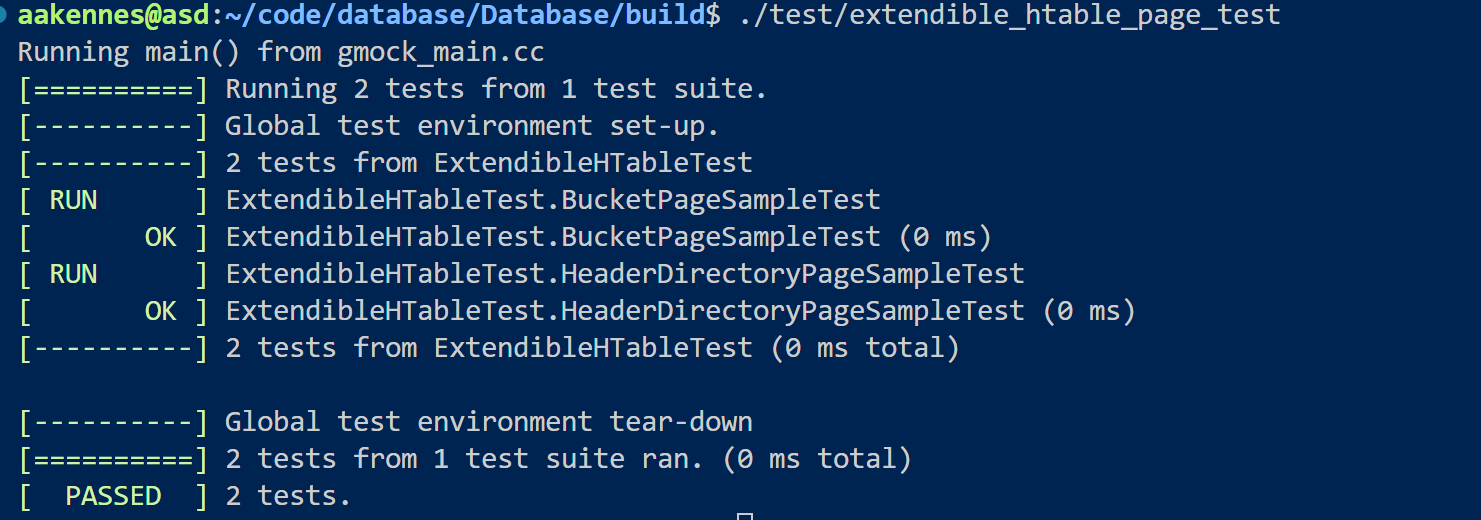
\includegraphics[scale=0.2]{19.png}
   \caption{Task1}
   \label{fig:1}
\end{figure}


\begin{figure}[h!]
   \centering
   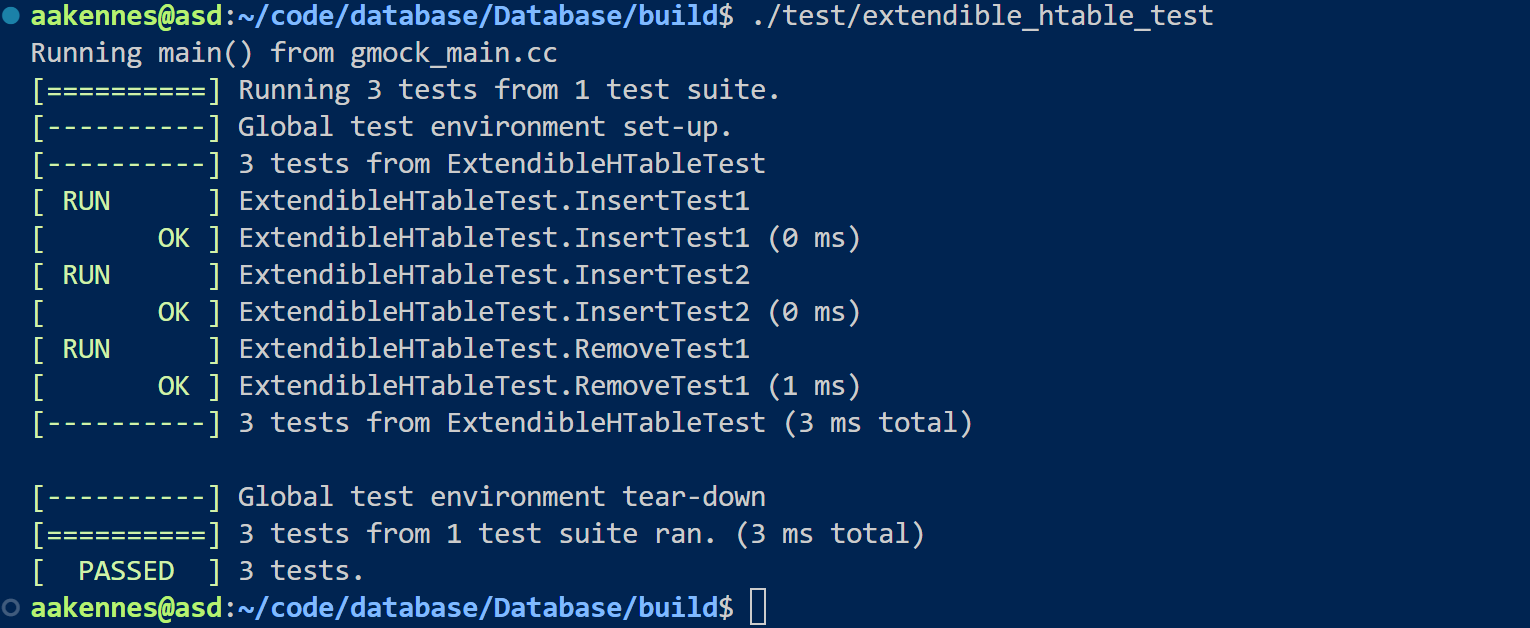
\includegraphics[scale=0.33]{20.png}
   \caption{Task2}
   \label{fig:1}
\end{figure}

\begin{figure}[h!]
   \centering
   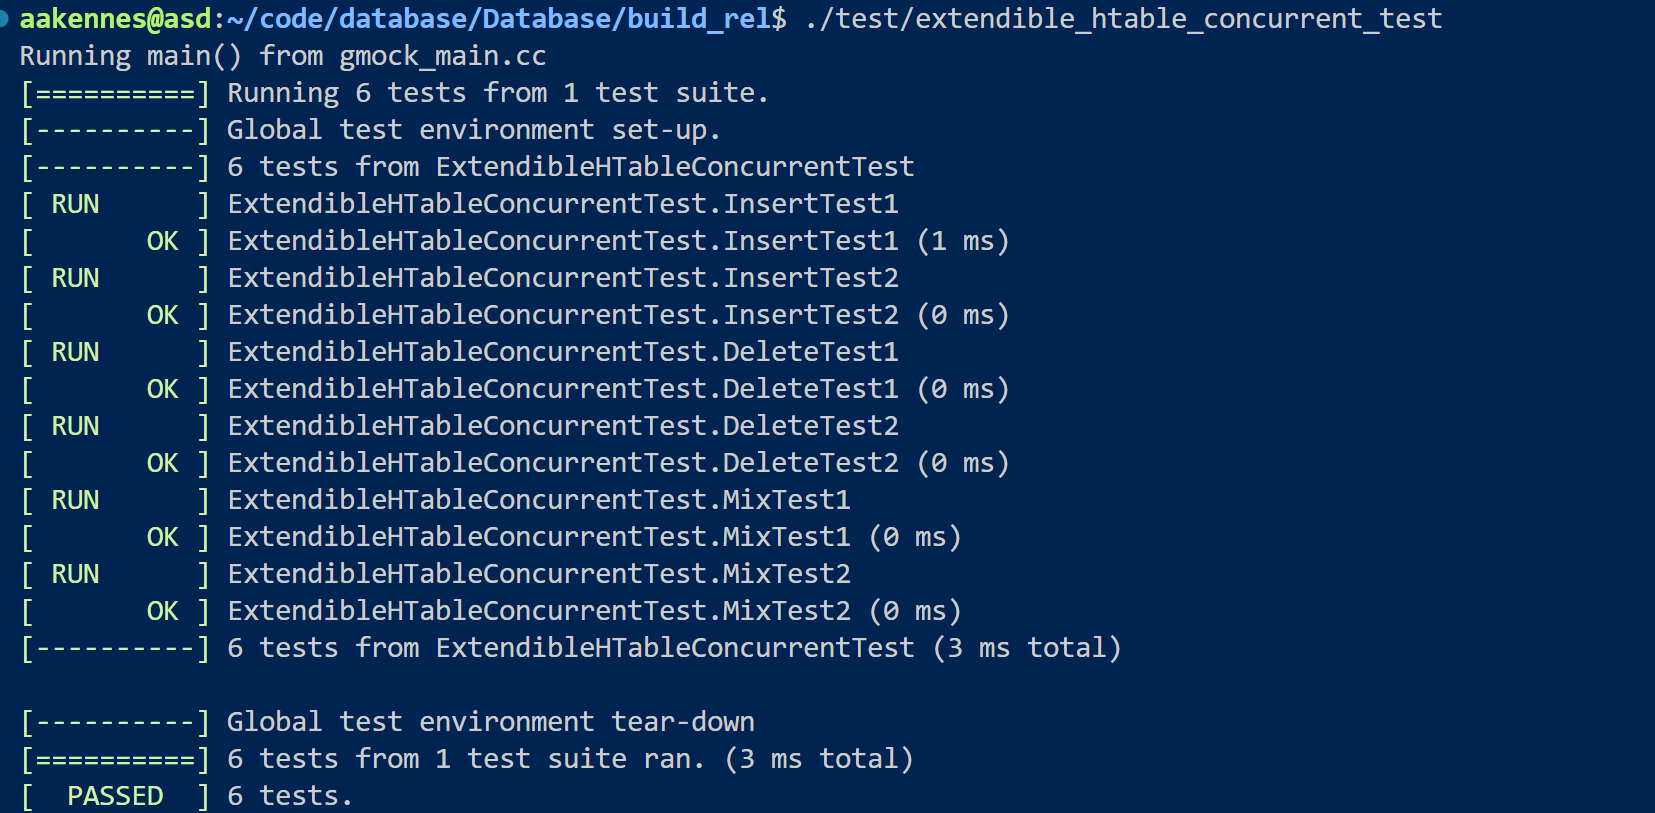
\includegraphics[scale=0.3]{21.png}
   \caption{Task3}
   \label{fig:1}
\end{figure}

\section{Protect2介绍}

\subsection{外部结构}

project2与project1联系紧密,主要需要我们实现可扩展哈希表(ExtendibleHashIndex),
数据库使用可扩展哈希表调用或调整每个读写页(Read/WritePage),需要注意的是我们在
可扩展哈希表中存储的是每个读写页在缓存池(BufferPoolManager)中的下标。

\begin{figure}[h!]
   \centering
   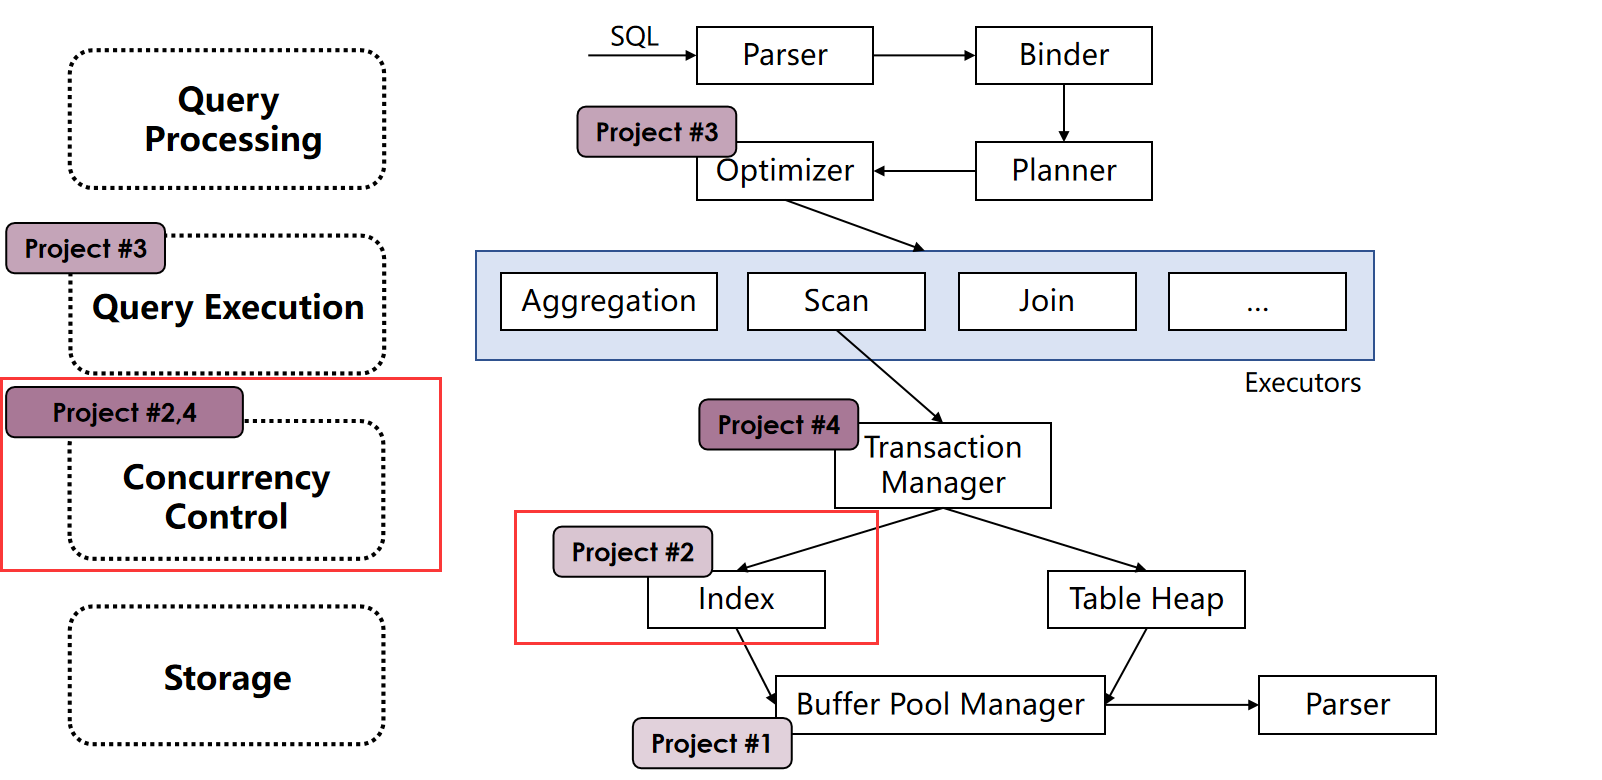
\includegraphics[scale=0.5]{2.png}
   \caption{Bustub的结构}
   \label{fig:1}
\end{figure}

相对于project1而言,project2主要代码在task2的插入删除的实现上,同时由于涉及到了
project1的读写页的插入删除,在调试上还需要考虑task1的问题。同时,由于每个.h文件中
注释过少,导致很多函数意义不明,尤其是task1的directory部分以及task2的从上级目录
访问下级目录的方法上。

可扩展哈希表一共有三级目录,在task1:Extendible Hash Table Pages中,我们会实现
三级目录(header,directory,bucket)内部的初始化,插入删除等更新维护操作,
在task2:Extendible Hashing Implementation中,我们会实现三级目录外部的
操作,完成一个页面(page)插入和删除到三级目录下的全过程。同时,在最后的Task3:
Concurrency Control中,我们需要使用缓存池中的读写锁(read/write\_page\_guard),
实现可扩展哈希表的并发控制。

\subsection{内部结构}

在开始下面整个project前,我们需要先理解整个可扩展哈希表的内部结构。

\begin{figure}[h!]
   \centering
   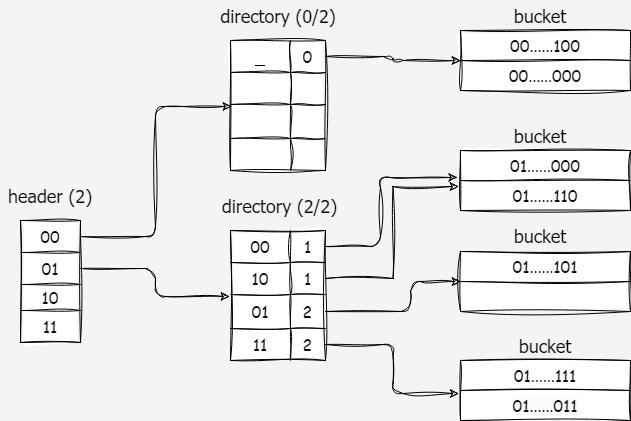
\includegraphics[scale=1]{1.png}
   \caption{ExtendibleHashTable的结构}
   \label{fig:1}
\end{figure}

查询一个键值对:第一关键字(key)和第二关键字(value)的过程如下:

\begin{enumerate}
   \item 获取第一关键字的哈希值hash
   \item 依据hash的前max\_depth位查询到hash对应的header
   \item 在当前的header中依据hash的后global\_depth位查询到hash对应的bucket
   \item 在当前的bucket中直接搜索到对应的hash值,将键值对插入到bucket中。
\end{enumerate}

具体的访问逻辑会在task2中具体介绍。

其中header的数目固定,directory和bucket的数目可以动态扩展和缩减。在图3.2中,
每一个大框代表着一个页面(page),header和directory页面(page)仅用来索引下一级目录,
bucket页面(page)用来存储实际键值对。

这里需要区分idx和page\_id的区别,以header中的directory\_idx和directory\_page\_id为例,
header中有数组directory\_page\_ids\_,directory\_idx是directory\_page\_ids\_的下标,
可以通过该数组和director\_idx下标索引到具体的page\_id,再通过缓存池中的函数,用page\_id索引到具体
到页面(page)。为了方便区分,下文将directory\_idx称作目录索引下标,将directory\_page\_id
称作目录页面下标。

同时,每一级目录都有一个数组array,header的数组directory\_page\_ids用来存储
唯一header指向的二级目录directory的目录页面下标,directory的数组bucket\_page\_ids用来存储
当前directory指向的三级目录bucket的目录页面下标。bucket的数组array用来存实际
存储的键对值。

下面分别介绍三层目录:

\subsubsection{header}

header是一个固定的页面(page),即一个可扩展哈希表只有一个标题页,可看作静态
一级目录页面,header的大小固定,为$2^{max_depth}$。

变量:
\begin{itemize}
   \item directory\_page\_ids\_:二级目录页面directory的页面(page)索引。
   \item max\_depth\_:header的深度。
\end{itemize}

函数:

\begin{itemize}
   \item HashToDirectoryIndex:哈希值转二级目录。
   \item GetDirectoryPageId:取得directory\_page的下标值。
   \item SetDirectoryPageId:设置directory\_page的下标值。
\end{itemize}

\subsubsection{directory}

directory是可扩展哈希表中最关键的部分,我们需要理解Global\_Depth和
Local\_Depth的作用以及二级目录directory是怎样索引到三级目录。

\begin{itemize}
   \item Global\_Depth:不同hash值的有效位为后Global\_Depth位,即在图3.3中,
   使用5位哈希值的后2位区分不同的哈希值。Global\_Depth的值决定了directory的目录大小,
   directory的目录大小为$2^{Global\_Depth}$。在索引一个bucket的目录索引下标时,只需要
   查看后Global\_Depth位,即一个哈希的bucket\_idx等于其值的后Global\_Depth位。
   \item Local\_Depth:在同一个bucket中,后Local\_Depth位均相等,等于
   其directory的后Local\_Depth位,Local\_Depth$\leq$Global\_Depth。
   一个bucket有$2^{Global\_Depth-Local\_Depth}$个指向它的指针。
\end{itemize}

\begin{figure}[h!]
   \centering
   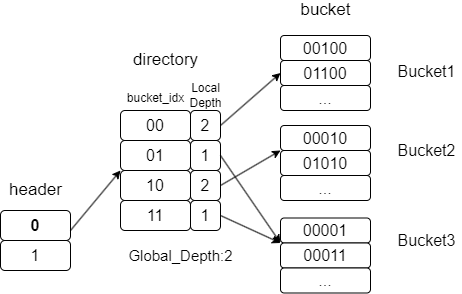
\includegraphics[scale=0.6]{3.png}
   \caption{directory和bucket的结构}
   \label{fig:1}
\end{figure}

注意,图中directory的下标为bucket\_idx目录索引下标,需要通过目录页面下标bucket\_page\_id访问页面(page)。
bucket的下标只代表bucket\_page的目录页面下标的相对顺序,不代表具体的目录页面下标bucket\_page\_id。
同一个bucket\_idx可以指向不同的bucket\_page\_id,如图3.2中目录2和4就指向了Bucket3。

除开了解二级目录directory的结构外,我们还应该理解插入删除过程中directory的
合并与分裂的全过程,这也是可扩展哈希表能够维护自身动态,减少内存消耗的关键。

变量:
\begin{itemize}
   \item max\_depth:GLobalDepth和LocalDepth的最大值
   \item bucket\_page\_ids:bucket的目录页面下标
   \item Global\_Depth,Local\_depths
\end{itemize}

函数:

\begin{itemize}
   \item GetGlobalDepthMask:掩值定义为取原哈希值的部分位,GlobalDepth的掩值用作
   将哈希值转换为bucket\_idx,因此数值为$(1 << global_depth_) - 1$
   \item GetLocalDepthMask:LocalDepth的掩值用作求bucket分裂(对应图2.4)后
   分裂出的bucket\_idx,数值为$1 << local_depths_[bucket_idx]$。
   \item HashToBucketIndex:将哈希值与上GlobalDepth的掩值即可得到bucket\_idx。
   \item GetSplitImageIndex:用来求directory分裂后的新bucket,即imagebucket,
   将bucket\_idx的第GlobalDepth-1位与1异或即可。
   \item IncrGlobalDepth,DecrGlobalDepth:在分裂和合并directory时要对GlobalDepth进行增减,
   除了直接对GlobalDepth进行操作外,还要更新bucket\_page\_ids和local\_depths
   \item CanShrink:判断directory能否合并,标准为所有的LocalDepth都小于GlobalDepth
   \item IncrLocalDepth,DecrLocalDepth:在分裂和合并bucket时要对LocalDepth进行增减,
   除了直接对LocalDepth进行操作外,还要更新imagebucket的LocalDepth。
   \item SetLocalDepth,GetLocalDepth,Size,GetGlobalDepth,Init
\end{itemize}

\subsubsection{bucket}

bucket用来存实际存储的健对值,在可扩展哈希中保证了一个key只会对应一个value。

变量:
\begin{itemize}
   \item array\_:存储的健对值,是一个pair数组。
   \item size\_:array\_的大小。
   \item max\_size\_:array\_的容量。
\end{itemize}

函数:

\begin{itemize}
   \item Lookup:查询一个关键字是否在这个bucket中。
   \item Insert:向当前bucket中插入一个键对值。
   \item Remove,RemoveAt:将bucket中删除key对应的键对值。
   \item KeyAt,ValueAt,EntryAt,SizeIsFull,IsEmpty
\end{itemize}

\subsection{directory的分裂}

当要插入的bucket满了(bucket的size=max\_size)时,我们要执行分裂操作:

\begin{enumerate}
   \item 判断directory内的bucket是否已满(Global\_Depth=当前bucket的Local\_Depth)。
   \item 若是,增加Global\_Depth,将directory内的bucket数量翻倍,imagebucket的下标为$2^{Global\_Depth-1}+1-2^{Global\_Depth}$
   ,是bucket$0-2^{Global\_Depth-1}$的复制,指向和Local\_Depth相同,这样就保证了一定会有多个指针
   指向同一个bucket,即一定有位置空给新增的bucket。
   \item 增大Local\_Depth,将已满的bucket一分为二,并按照后Local\_Depth位(local\_depth\_mask)的不同
   将对应元素填入bucket和imagebucket中,分裂后需要更新Local\_Depth和两个bucket的指向。
\end{enumerate}

分裂前后的bucket\_idx的第Global\_Depth位互补,这也是GetSplitImageIndex函数
要我们求的东西,本project中将分裂后的bucket称为imagebucket,具体可参考图2.5到图2.6中
directory的转化。

以下分别是两种分裂类型。

\begin{figure}[h!]
   \centering
   \subfigure[找到插入位置判断bucket已满]{
      \begin{minipage}[t]{0.33\linewidth}
      \centering
      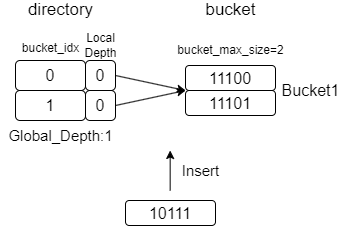
\includegraphics[width=2in]{4.png}
      \label{fig:diff1}
      \end{minipage}%
   }%
   \subfigure[分裂]{
      \begin{minipage}[t]{0.33\linewidth}
      \centering
      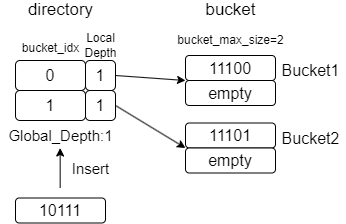
\includegraphics[width=2in]{5.png}
      \end{minipage}%
   }%
   \subfigure[插入到新bucket]{
      \begin{minipage}[t]{0.33\linewidth}
      \centering
      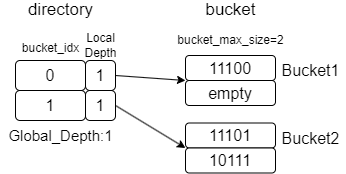
\includegraphics[width=2in]{6.png}
      \end{minipage}%
   }%
   \centering
   \caption{插入10111,只分裂bucket}
   \label{fig:diff}
\end{figure}

\begin{figure}[h!]
   \centering
   \begin{minipage}[b]{0.4\linewidth}
     \centering
     \begin{subfigure}{}
       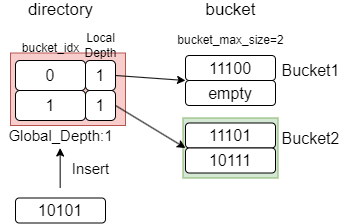
\includegraphics[width=\linewidth]{9.png}
       \caption{判断bucket已满进行bucket的分裂}
     \end{subfigure}
     \vfill
     \begin{subfigure}{}
       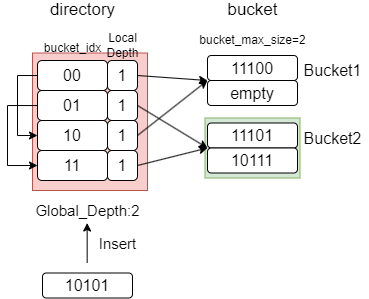
\includegraphics[width=\linewidth]{10.png}
       \caption{比较GD和LD并进行directory的分裂}
     \end{subfigure}
   \end{minipage}%
   \begin{minipage}[b]{0.4\linewidth}
     \centering
     \begin{subfigure}{}
       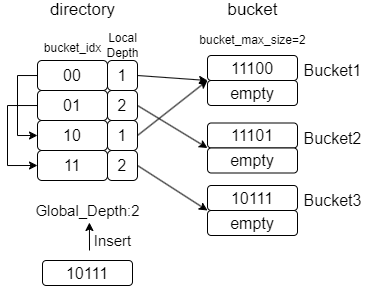
\includegraphics[width=\linewidth]{11.png}
       \caption{更新Local\_Depth和指向}
     \end{subfigure}
     \vfill
     \begin{subfigure}{}
       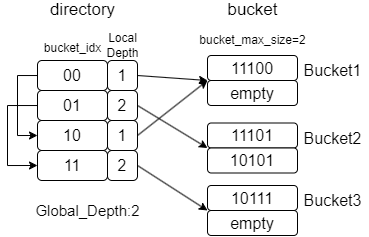
\includegraphics[width=\linewidth]{12.png}
       \caption{插入到新bucket}
     \end{subfigure}
   \end{minipage}
   \caption{插入10101,要分裂directory和bucket}
 \end{figure}



\subsection{directory的合并}

合并操作实际上就是将整个分裂过程反过去,当bucket已满时分裂,当bucket已空的时候合并:

\begin{enumerate}
   \item 减少Local\_Depth,将已空的bucket合二为一,并按照后Local\_Depth位(local\_depth\_mask)的不同
   将imagebucket的元素填入newbucket中,并删除imagebucket。合并后需要更新Local\_Depth和bucket的指向。
   \item 判断directory内的所有bucket的Local\_Depth都小于Global\_Depth(can\_shrink)。
   \item 若是,减少Global\_Depth,将directory内的bucket数量减一半,合并后的newbucket的指向和Local\_Depth与bucket和imagebucket中下标最小的相同,
   保证最后指向的bucket为合并后的newbucket。
\end{enumerate}

\begin{figure}[h!]
   \centering
   \begin{minipage}[b]{0.4\linewidth}
     \centering
     \begin{subfigure}{}
       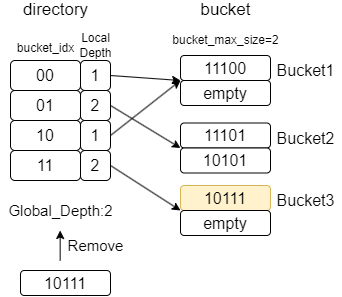
\includegraphics[width=\linewidth]{13.png}
       \caption{找到删除位置直接删除}
     \end{subfigure}
     \vfill
     \begin{subfigure}{}
       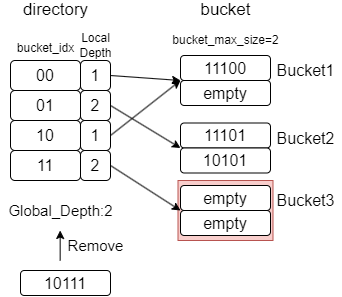
\includegraphics[width=\linewidth]{14.png}
       \caption{判断bucket为空进行bucket的合并}
     \end{subfigure}
   \end{minipage}%
   \begin{minipage}[b]{0.4\linewidth}
     \centering
     \begin{subfigure}{}
       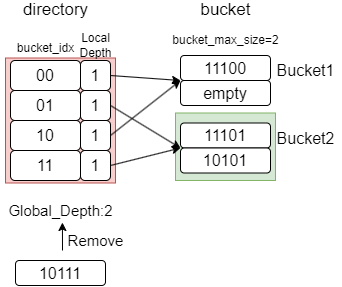
\includegraphics[width=\linewidth]{15.png}
       \caption{比较GD和LD并进行directory的合并}
     \end{subfigure}
     \vfill
     \begin{subfigure}{}
       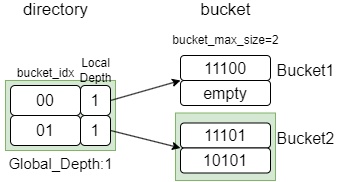
\includegraphics[width=\linewidth]{16.png}
       \caption{更新指向和Local\_Depth}
     \end{subfigure}
   \end{minipage}
   \caption{删除10111,要合并directory和bucket}
 \end{figure}

需要注意的是,不管是分裂还是合并操作,都需要循环分裂/合并直到bucket不满/空为止。

\begin{figure}[h!]
   \centering
   \subfigure[多次分裂]{
      \begin{minipage}[t]{0.5\linewidth}
      \centering
      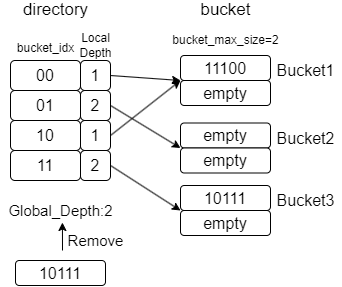
\includegraphics[width=2in]{17.png}
      \label{fig:diff1}
      \end{minipage}%
   }%
   \subfigure[多次合并]{
      \begin{minipage}[t]{0.5\linewidth}
      \centering
      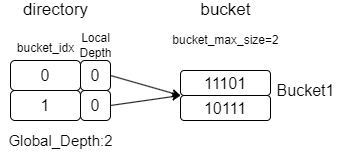
\includegraphics[width=2in]{18.png}
      \end{minipage}%
   }%
   \caption{循环分裂合并}
   \centering
   \label{fig:diff}
\end{figure}

\section{Task1:Extendible Hash Table Pages}

\subsection{header}

header的函数实现较为简单,不作赘述。

\subsection{directory}

在上一个部分已经详细介绍了各个变量和函数的作用,重点实现下面的函数:

\begin{itemize}
   \item Init:bucket\_page\_ids\_数组中的每个值要初始化为INVALID\_PAGE\_ID(=-1)。
   \item GetSplitImageIndex:bucket\_idx的第GlobalDepth-1位与1异或。
   \item HashToBucketIndex:哈希值与上global\_depth\_的掩值。
   \item IncrGlobalDepth:imagebucket的local\_depths\_和bucket\_page\_ids\_初始化为oldbucket的。
   \item DecrGlobalDepth:imagebucket的local\_depths\_和bucket\_page\_ids\_设置为空(0和-1).
   \item CanShrink:local\_depths\_都小于global\_depths\_。
   \item SetLocalDepth:虽然在local\_depths\_task2中,local\_depths\_的增减幅度一定为1,但是
   初始化过程中可能存在比1大的情况,所以需要将local\_depths\_循环单次增减到指定的值。
   \item IncrLocalDepth/DecrLocalDepth:imagebucket的local\_depths\_也需要增减。
\end{itemize}

\subsection{bucket}

bucket的函数实现需要知道比较函数是自定义的,比较两个键对值需要使用传入的cmp\_
函数,返回值为0代表两个第一关键字相等。重点实现下面的函数:

\begin{itemize}
   \item Init:除了初始化size\_和max\_size\_外,需要对array\_数组中的每一个键对
   进行初始化,key和value的数据类型都是模板,其中value有默认的构造函数,采取下面的初始化方式:
   \begin{minted}[mathescape,
      linenos,
      numbersep=5pt,
      gobble=2,
      frame=lines,
      framesep=2mm,
      highlightcolor=green!40]{cpp}
      K ktemp = {-1};
      V vtemp = {};
      array_[i] = std::make_pair(ktemp, vtemp);
   \end{minted}
   \item Insert:可扩展哈希表要求每个key都不同,不允许插入相同元素,所以需要先判断插入的key是否存在,存在就返回false。
   \item Remove:array\_数组要求连续,所以没删除一个元素后需要将被删除元素后的数组整体往前移一位。
\end{itemize}

\subsection{Debug}

注意每个数组的下标都是从0开始,所以大小为size的数组,下标最大值为size-1,遍历
的时候需要考虑枚举的上限。

\section{Task2:Extendible Hashing Implementation}

重点实现的函数为Insert和Remove函数,在上一部分已粗略的介绍了简要逻辑下面将
展示具体的伪代码。

在开始可扩展哈希表的插入删除前,我们要知道怎么从上级目录访问或新建下级目录,
由于缺失相关资料,这一部分主要参考自task1中的测试样例的访问方法。

已知的是上级目录的目录页面id,以directory\_page\_id为例,使用缓存池中已实现的page\_guard对head\_page
进行定位。

\begin{enumerate}
   \item 将key的哈希值转换为directory\_page\_index
   \item 使用header\_page的GetDirectoryPageId函数将目录索引下标转换为目录页面id,若没有在header\_page中找到,说明不存在,此时要将bucket插入到一个新的directory内。
   \item 使用FetchPageRead/Write/NewPageGuarded获取directory\_page\_guard
   \item 使用directory\_page\_guard中的As/Asmut函数定位到具体的bucketpage
   \item 在page使用完后,使用Drop()。
\end{enumerate}

As与Asmut的区别是只读和可写入的区别,所以FetchPageRead对应As,FetchPageWrite和NewPageGuarded对应Asmut。

\subsection{Insert}

InsertToNewDirectory和InsertToNewBucket的实现较为简单,注意插入到新的directory后也需要插入到新的bucket,
下为Insert的伪代码:
\begin{breakablealgorithm} 
  \caption{向可扩展哈希表中插入一个<key,value>} 
  \begin{algorithmic}[1] %每行显示行号  
      \Require 插入成功返回true,否则为false
      \Function {Insert}{$key,value$}
           \State $header\_page \gets header\_get()$$//$使用上面介绍的方法获得$header\_page$
           \State $directory\_page\_index,directory\_page\_id \gets HashToDirectoryIndex(),GetDirectoryPageId()$
           \State $//$分别获得$index$和$id$
           \If {$directory\_page\_id = INVALID\_PAGE\_ID $}
             \State $insert_success \gets InsertToNewDirectory()$
             \State\Return{$insert_success$}
           \EndIf
           \State $directory\_page \gets directory\_get()$
           \State $bucket\_page\_index,bucket\_page\_id \gets HashToBucketIndex(),GetBucketPageId()$
           \If {$bucket\_page\_id = INVALID\_PAGE\_ID $}
             \State $insert_success \gets InsertToNewBucket()$
             \State\Return{$insert_success$}
           \EndIf
           \State $bucket\_page \gets bucket\_get()$
           \While {$bucket\_page$为满}
             \If {$local\_depth = global\_depth $}
               \If{$global\_depth = directory\_max\_depth$}
                 \Return{false}
                 \State $//$已达到最大,无法扩展
               \EndIf
               \State $directory\_page->IncrGlobalDepth()$
               \State $directory\_page \gets directory\_get()$
               \State $//$更新GlobalDepth和directorypage
               \State $bucket\_page\_index,bucket\_page\_id \gets HashToBucketIndex(),GetBucketPageId()$
               \State $//$更新bucket和directorypage,id为空时要调用$InsertToNewBucket()$
             \EndIf
             \State $directory\_page->IncrLocalDepth()$
             \State $new\_bucket\_page \gets new\_buckey\_get()$
             \State $new\_bucket\_idx \gets bucket\_idx \oplus local\_mask$
             \For{i = 0 to bucket\_size}
               \State $new\_bucket\_page->Insert()$
               \State $bucket\_page->Remove()$
               \State $//$按local\_mask分开两个bucket
             \EndFor
             \State $bucket\_page \gets bucket\_get()$
             \State $directory_page->SetBucketPageId(bucket\_idx, bucket_page\_id)$
             \State $//$更新分裂后的bucket和directory的索引
           \EndWhile
           \State $insert\_success = bucket\_page->Insert(key, value)$
           \State 若插入成功还需要更新$directory\_page->SetBucketPageId(bucket\_idx, bucket_page\_id)$
           \Return{$insert\_success$}
      \EndFunction
  \end{algorithmic}  
\end{breakablealgorithm}

\subsection{Remove}

\begin{breakablealgorithm} 
  \caption{在可扩展哈希表中删除key对应的键对} 
  \begin{algorithmic}[1] %每行显示行号  
      \Require 删除成功返回true,否则为false
      \Function {Remove}{$key$}
        \State $header\_page \gets header\_get()$
        \State $directory\_page\_index,directory\_page\_id \gets HashToDirectoryIndex(),GetDirectoryPageId()$
        \State $directory\_page \gets directory\_get()$
        \State $bucket\_page\_index,bucket\_page\_id \gets HashToBucketIndex(),GetBucketPageId()$
        \State $bucket\_page \gets bucket\_get()$
        \State $remove\_success \gets bucket\_page->Remove(key)$
        \If{$remove\_success = false$}
          \State $false$ $//$代表删除失败
        \EndIf
        \While {$bucket\_page$为空}
          \If {$local\_depth = global\_depth $}
            \If{$global\_depth = 0$}
              \State $directory\_page->SetBucketPageId(bucket\_idx, INVALID\_PAGE\_ID)$
              \Return{true} $//$已达到最小,无法合并
            \EndIf
            \State $image\_bucket\_idx,image\_bucket\_page\_id \gets GetSplitImageIndex(),GetBucketPageId()$
            \If{$image\_bucket_idx > bucket\_idx$}
              \State $//$imagebucket比bucket大,说明要把imagebucket的元素插入到bucket中
              \State $image\_bucket\_page \gets image\_bucket\_get$
              \For{i = 0 to image\_bucket\_size}
                \State $bucket\_page->Insert()$
                \State $image\_bucket\_page->Remove()$
              \EndFor
              \State $bpm\_->DeletePage(new\_bucket\_page\_id)//$删除页面
            % \EndIf
            \Else
              \State $bpm\_->DeletePage(bucket\_page\_id)$
              \State $bucket\_idx \gets image\_bucket\_idx//$转换bucket
            \EndIf
            \State $directory\_page->DecrLocalDepth$
          \EndIf
          \State $directory\_page->IncrLocalDepth()$
          \If{$CanShrink$}
            $directory\_page->DecrGlobalDepth()$
          \EndIf
          \State $bucket\_page \gets bucket\_get()$
          \State $//$更新分裂后的bucket
        \EndWhile
        \Return{$true$}
      \EndFunction
  \end{algorithmic}  
\end{breakablealgorithm}

\subsection{Debug}

\begin{itemize}
   \item 插入的分裂操作中,在bucket分裂涉及到了bucketpage中有选择的删除元素,此时要注意循环枚举的i,避免出现访问到悬空指针的情况,
   这一问题类似set/vector等容器的删除。
   \item Remove中要对删除的page在缓存池中进行删除,否则会造成空间浪费,注意shrink后不能
   将imagebucket进行删除,因为canshrink就保证了bucket和imagebucket指向同一个bucket。
   \item 由于bucketpage中key,value和cmp都是模板,在Asmut函数里要加上<K,V,KC>。
   \item 合并操作中,imagebucket与bucket哪个大代表要删除哪个bucket,所以在删除bucketpage时要判断一下。
\end{itemize}

\section{Task3:Concurrency Control}

在task2中实现读写锁就是实现了并发控制,注意及时对无用的page进行drop(),否则可能发生死锁或线程冲突。

\subsection{Debug}

由于涉及到了缓存池中的page\_guard,所以该task出错的原因不止是未及时drop()导致的线程冲突,
还有可能是task3和task4中的锁的问题和dirty标记的设置问题。

\begin{itemize}
   \item 锁的问题,采取了unique\_lock,在调用有锁的函数前进行解锁,函数结束后加锁
   ,调试时还发现Read/WritePage函数里也有锁。
   \item UnpinPage中dirty标记更新有误导致出现了线程问题,只有当dirty标记为1时才对要更新的dirty进行更新,为0时不更新。
\end{itemize}


\newpage
\bibliographystyle{plain}
\bibliography{reference.bib} 

\end{document}